\documentclass[a4paper, 12pt]{article}
\usepackage[T2A]{fontenc} 
\usepackage[utf8]{inputenc}
\usepackage[english,russian]{babel} 


\usepackage{amsmath,amsfonts,amssymb,amsthm,mathtools}

\usepackage[left=2cm,right=2cm,top=2cm,bottom=2cm,bindingoffset=0cm]{geometry}

\usepackage{graphicx}

\newtheorem*{theorem}{Теорема}
\newtheorem*{corollary}{Следствие}
\newenvironment{Proof}
{\par\noindent{$\blacklozenge$}}
{\hfill$\scriptstyle\boxtimes$}

\usepackage[normalem]{ulem}
\usepackage[unicode]{hyperref}

\newcommand{\R}{\mathbb{R}}
\renewcommand{\C}{\mathbb{C}}
\renewcommand{\Re}{\operatorname{Re}}
\renewcommand{\Im}{\operatorname{Im}}
\renewcommand{\leq}{\leqslant}
\renewcommand{\geq}{\geqslant}

\title{\vspace{6.5cm}\textbf{\Huge{Алгебра и Теория чисел}}\\Конспект по 1 семестру 
специальности «прикладная информатика»\\(лектор Г. В. Матвеев)}
\date{}
\begin{document}
\maketitle
\newpage
\tableofcontents{}
\newpage

\section{Операции над комплексными числами}
Множество комплексных чисел имеет вид:
$$\C=\{a+bi \: |\ a,b \in \R \},$$
где число $i$ --- мнимая единица.\\\\
По определению $i^2=-1$\\\\
$\bullet$ \textit{\textbf{Общим видом} комлексного числа называется представление}
$$z = a + bi$$
$\bullet$ \textit{Число $a = \Re z$ --- \textbf{вещественная} часть числа $z$}.\\
$\bullet$ \textit{Число $b = \Im z$ --- \textbf{мнимая} часть числа $z$.}\\\\
\textit{\textbf{Операции над комплексными числами:}}\\
\begin{enumerate}
    \item \textit{Сложение и вычитание комплексных чисел}
    $$(a+bi) \pm (c+di) = (a \pm c) + (b \pm d)\cdot i.$$
    \item \textit{Сравнение комплексных чисел}
    $$a+bi = c+di \Longleftrightarrow \begin{cases} a = c,\\ b = d. \end{cases}$$
    \item \textit{Нулевое комплексное число}
    $$a + bi = 0 \Longleftrightarrow \begin{cases} a = 0,\\ b = 0. \end{cases}$$
    \item \textit{Умножение комплексных чисел}
    $$(a+bi)\cdot (c+di)=(ac-bd)+(ad+bc)\cdot i.$$
    \item \textit{Деление комплексных чисел}
    $$\frac{a+bi}{c+di} = \frac {(a+bi)\cdot (c-di)}{(c+di)\cdot (c-di)} = \frac {ac+bd}{c^2+d^2}+\frac{bc-ad}{c^2+d^2}\cdot i.$$
\end{enumerate}
\textit{\textbf{Свойства сложения и умножения:}}
\begin{enumerate}
    \item \textit{Коммутативность}
    $$z_1 + z_2 = z_2 + z_1;$$
    $$z_1\cdot z_2=z_2\cdot z_1.$$
    Коммутативность комплексных чисел вытекает из коммутативности вещественных.
    \item \textit{Ассоциативность}
    $$z_1 + (z_2 + z_3) = (z_1 + z_2) + z_3;$$
    $$z_1\cdot (z_2\cdot z_3)=(z_1\cdot z_1)\cdot z_3.$$
    \item \textit{Существование противоположного числа}
    $$\forall z\ \exists (-z), \: z+(-z)=0.$$
    \item \textit{Дистрибутивность}
    $$z_1\cdot (z_2+z_3)=z_1\cdot z_2+z_1\cdot z_3.$$
\end{enumerate}
\subsection{Геометрическая интерпретация комплексных чисел}
$\bullet$ \textit{Число $\overline{z}=a-bi$ называется \textbf{сопряженным числом} для числа $z=a+bi$}.\\
\begin{figure}[ht]
\centering
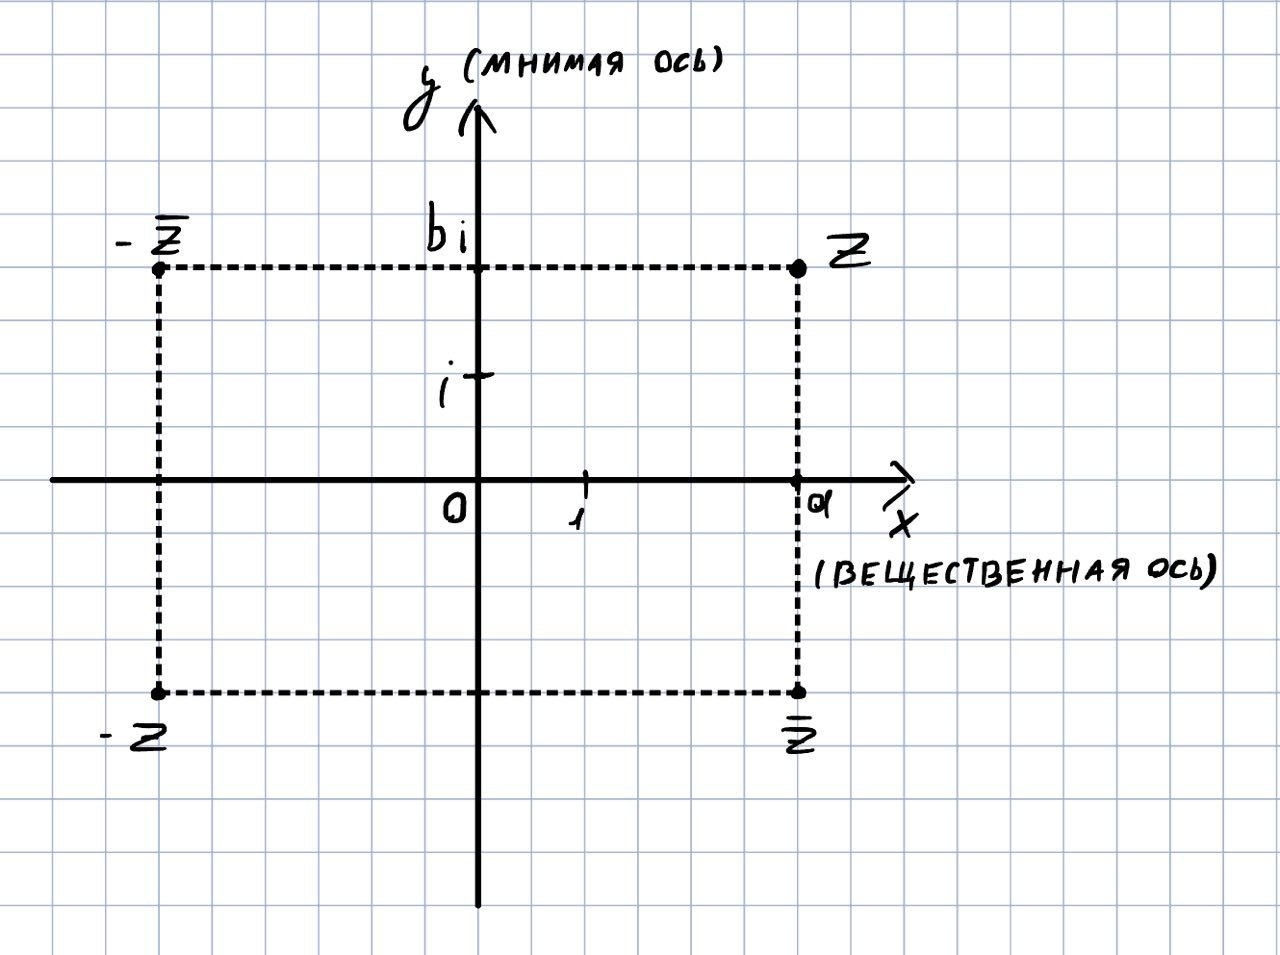
\includegraphics[width=0.5\linewidth]{pict1.jpg}
\caption{Комплексные числа на плоскости}
\label{fig:reg}
\end{figure}\\
\textit{\textbf{Свойства сопряженных чисел:}}
\begin{enumerate}
    \item $\overline{\overline{z}}=z$.
    \begin{Proof}
        $\overline{\overline{a+bi}} = \overline{a-bi} = a+bi = z$.
    \end{Proof}
    \item $\overline{z_1+z_2} = \overline{z_1}+\overline{z_2}$.
    \begin{Proof}
        $\overline{z_1+z_2}=\overline{a+bi+c+di}=\overline{(a+c)+(b+d)\cdot i} = (a+c)-(b+d)\cdot i$;\\
        $\overline{z_1}+\overline{z_2}=a-bi+c-di=(a+c)-(b+d)\cdot i=\overline{z_1+z_2}.$
    \end{Proof}
    \item $\overline{z_1 \cdot z_2}=\overline{z_1}\cdot\overline{z_2}$.
    \begin{Proof}
        $\overline{z_1}\cdot\overline{z_2}=(a-bi)(c-di)=(ac-bd)-(ad+bc)\cdot i$;\\
        $z_1\cdot z_2=(a+bi)(c+di)=(ac-bd)+(ad+bc)\cdot i$;\\
        $\overline{z_1\cdot z_2} = (ac-bd)-(ad+bc)\cdot i = \overline{z_1}\cdot\overline{z_2}.$
    \end{Proof}
    \item $\overline{\Big(\dfrac{z_1}{z_2}\Big)} = \dfrac{\overline{z_1}}{\overline{z_2}}.$
    \begin{Proof}
        $\dfrac{z_1}{z_2}=\dfrac{a+bi}{c+di}\cdot \dfrac{c-di}{c-di}=\dfrac{ac+bd}{c^2+d^2}+\dfrac{bc-ad}{c^2+d^2}$;\\\\
        $\overline{\Big(\dfrac{z_1}{z_2}\Big)}=\dfrac{ac+bd}{c^2+d^2}+\dfrac{ad-bc}{c^2+d^2}\cdot i$;\\\\
        $\dfrac{\overline{z_1}}{\overline{z_2}}=\dfrac{a-bi}{c-di} \cdot \dfrac{c+di}{c+di} = \dfrac{ac+bd}{c^2+d^2}+\dfrac{ad-bc}{c^2+d^2}\cdot i = \overline{\Big(\dfrac{z_1}{z_2}\Big)}.$
    \end{Proof}
    \item $z\cdot \overline{z} = (a+bi)\cdot (a-bi)=a^2+b^2.$
\end{enumerate}
$\bullet$ \textit{\textbf{Модулем} комплексного числа называется число}
$$|z|=\sqrt{a^2+b^2}=\sqrt{z\cdot\overline{z}}, \quad |z| \in \R.$$
\textit{\textbf{Свойства модуля:}}
\begin{enumerate}
    \item $|z_1\cdot z_2|=|z_1|\cdot |z_2|$;
    \item $|z_1+z_2| \leq |z_1| + |z_2|$;
    \item $z=0 \Longleftrightarrow |z|=0$.
\end{enumerate}

\end{document}
